\documentclass[12pt,a4paper,titlepage]{article}
%\usepackage[doublespacing]{setspace}
\usepackage[utf8]{inputenc}         %This is used for ASKII digits.
\usepackage{amsmath, amssymb}       %This is for mathematic statements,check"amath.colorado.edu/documentation/LaTex/Symbols.pdf"
\usepackage{booktabs}
\usepackage{caption2}
\usepackage{epstopdf}
\usepackage{amsfonts,mathrsfs}      %fonts~~
\usepackage{graphicx}               %This is for graph inserting.
\usepackage{paralist}               %Give me compact lists!!!!! 'compactitem' 'compactenum' 'compactdesc'
%\usepackage{bm}                     %various kinds of bold texts.
\usepackage[top =2.54cm, bottom =2.54cm, left =3.18cm, right =3.18 cm]{geometry}
\usepackage{indentfirst}            %Indent the first letter
\usepackage{fancyhdr}               %Below is the head of the article.
\pagestyle{fancy}
\usepackage{lastpage}
\lhead{Team \# 33131}
\rhead{Page \thepage{} of \pageref{LastPage}}
\cfoot{}
%\numberwithin{equation}{section}    %Numbering of the equations will be based on sections.
%\usepackage{amsthm}
%\theoremstyle{definition}
%\newtheorem{def}{Definition}  %Below set the theorem system.
%\theoremstyle{plain}
%\newtheorem{thm}[law]{Thm}
%\theoremstyle{remark}
%\newtheorem*{remark}{Remark}
\newcommand{\boldit}[1]{\textbf{\textit{#1}}}
\renewcommand{\captionlabelfont}{\small \bfseries \rmfamily}
\usepackage{float}
\usepackage{paralist}
\usepackage{url}

\begin{document}

\title{Human Capital Model} \date{\today{}}
\maketitle

\tableofcontents

\newpage

\section{Introduction}
\label{sec:introduction}

Considering the shortage of the talent, it's essential for companys to
retain good people and make them well-trained. However, current
situation is not satisfactory while many talents always tend to get a
good job via job-hopping, causing orgnizational churn in employees who
are closely connected to them. In order to simulate this process and
improve it, we build a human capital model based on Social Network
Analysis and Markov process.

\begin{displaymath}
Q=\iiint\limits_{\Omega}\rho C_{w}(u_f - u_i)dx dy dz
\end{displaymath}

\begin{displaymath}
\begin{aligned}
\int_{t_1}^{t_2} \iint\limits_{\Gamma}k\frac{\partial u}{\partial n}dsdt & =\iiint\limits_{\Omega}\rho C_{w}(u_f - u_i)dx dy dz\\
& =\int_{t_1}^{t_2}\iiint\limits_{\Omega}[\frac{\partial}{\partial x}(k\frac{\partial u}{\partial x})+\frac{\partial}{\partial y}(k\frac{\partial u}{\partial y})+\frac{\partial}{\partial z}(k\frac{\partial u}{\partial z})]dxdydx\\
& = \iiint\limits_{\Omega}\rho C_{w}(\int_{t_1}^{t_2}\frac{\partial u}{\partial t}dt)dxdydz
\end{aligned}
\end{displaymath}

\begin{displaymath}
\rho C_{w}\frac{\partial u}{\partial t}=k\bigtriangleup u+\frac{C_w V_h(u_h-u)}{}
\end{displaymath}

\subsection{Restatement of the Problem}
\label{sec:restatement-of-the-problem}
We are required to build a mathematical model to solve the problem of heating water in bathtub. Thus we have some subproblems:
\begin{itemize}
\item Build a basic model that demonstrate the change of the temperature in the bathtub in space and time without other intervention.
\item Figure out the influence of parameters such as the shape of the bathtub or the motions made by the person or so.
\item Propose a strategy to keep the temperature as even as possible.
\end{itemize}
In the first step, we build the simplest model. The shape of the bathtub is a cuboid, and the person will stay still. In the second step, the person move slowly and the shape of the bathtub changes. In the third step, we develop the conclusion of the  strategy.
\subsection{Literature Review}
\label{sec:literature-review}

\begin{itemize}
\item
\item
\item
\end{itemize}

\section{Terminology}
\label{sec:terminology}

\begin{itemize}
\item
\item
\item
\end{itemize}

\section{Assumptions and Justifications}
\label{sec:assumptions-and-justifications}

\begin{itemize}
\item \textbf{assumption 1} If an employee has probability to
  promote, he won't churn.

The possibility of the unforeseen accidents, which could force an
employee to leave his position,is neglected.Human nature, an employee
will stay at his position to chase for higher level.

\item \textbf{assumption 2} For a vacancy,if there exists an
  employee measures up to it already,ICM won't recruit for it.

Since recruiting good people is difficult, time consuming and
expensive according to issue 5,it is wasteful to recruit for a
position if an employee can promote to it.

\item \textbf{assumption 3} Demotion won't occur.

\item \textbf{assumption 4} Administrative clerk won't promote or be
  transferred.

\item \textbf{assumption 5} For the promotion probability and
  organization change, the other factors effects the churn probability
  is invariable.

Though churn derives from varieties of reasons and they are actually
lacking of known conditions and data to estimate them, we have to
regard it as stable in our model.

\item \textbf{assumption 6} Each division or office have at least one
  middle manager or senior manager.

\end{itemize}

% the main section of the paper
\section{Human Capital Model}
\label{sec:human-capital-model}

\subsection{Model Overview}
\label{sec:model-overview}

Partial differential equations are widely used in natural science, engineering and economical management.
It is natural to use partial differential equation to solve this physical problem.

In our model, five parts accounts for heat transfer of water: heat exchange between water and air, heat
exchange between water and the person, heat exchange between water and the bathtub, heat of hot water from the
faucet and heat of water flow outside. According to thermology, we conduct the equation
of water temperature in the bathtub. The initial-boundary value condition could be conducted according to
Fourier theorem, vaporization equation[ ].

Since the equation is a relatively complex 3D partial differential equation, we use matlab to solve it.
We build a geometry as the bathtub. By finite element method, the geometry discrete into several parts.
The solution of each part is considered to be a relatively precise value solution.

Definitions of symbols employed in this paper are listed in
\textbf{Table 1}.
\begin{table}
\begin{tabular}{l|l}
  Constant & Description \\
  \hline
  $k$            &Thermal conductivity of water \\
  $\rho$         &Density of water \\
  ${\gamma}_1$   &Heat exchange coefficient between water and air \\
  ${\gamma}_2$   &Heat exchange coefficient between water and person \\
  ${\gamma}_3$   &Heat exchange coefficient between water and bathtub \\
  $C_w$          &Specific heat capacity of water \\
  $V$            &Total volume of water \\
  $x_s$          &Humidity ratio in saturated air \\
  $x_0$          &Initial humidity ratio in the air \\
  $A$            &Square of water surface \\
  $V_a$          &Volume of surrounding air \\
  $C_v$          &Evaporation heat of water \\
  $u_2$          &Temperature of person's surface \\

  Variable & Description \\
  \hline
  $u$            &Temperature of water \\
  $u_1$          &Temperature of air \\
  $u_3$          &Temperature of bathtub \\
\end{tabular}
\end{table}

\subsection{Heat Equation}
\label{sec:heat equation}

In this part, we use physical theorem to conduct the heat conduction equation
in the bathtub.

Figure 1 shows thermal analysis of water in bathtub.

First,we assume that the heat change of all water in a tiny time $\Delta t$ is $\Delta Q$.
As shown in Figure 1, water in the bathtub have heat exchange with air, the person, and the bathtub.
In addition, heat changes when the hot water flow in and the excess water flow out.
Thus $\Delta Q$ is divided into five parts, i.e.
\begin{equation}
 \Delta Q=\Delta Q_1+\Delta Q_2-\Delta Q_3-\Delta Q_4
\end{equation}
in which $\Delta Q_1$ is heat transferred from air, person and bathtub,
$\Delta Q_2$ is the heat of the hot water from the faucet in $\Delta t$,
$\Delta Q_3$ is the heat of the water flow away in $\Delta t$,
$\Delta Q_4$ is the heat loss of vaporization.

Totally, internal energy of water changes while heat changes.
Then the temperature changes with
\begin{equation}
 1
\end{equation}

Considering the right side of equation 1.
Fourier theorem indicates that,
\begin{equation}
 dQ=-k\frac{\vartheta u}{\vartheta n}dSdt
\end{equation}
holds for the heat flow along a surface with square of dS.
In the equation, k is thermal conductivity, $\frac{\vartheta u}{\vartheta n}$
is the derivative of u along the normal line. Thus, after integration of dQ by time and
space
\begin{equation}
 \Delta Q_1=int_{t_1}^{t_2}[{int_{\Gamma}}k\frac{\vartheta u}{\vartheta n}dS]dt
\end{equation}
The heat flow into the water by thermal conduction could be calculated by this equation.

$\Delta Q_2$ is determined by the internal energy of hot water from the faucet in $\Delta t$.
And $\Delta Q_2$ can be calculated by
$\Delta Q_2={\Delta m}C{u_h}$.
Since the hot water is constant,
$\Delta m=v{\Delta t}$.

It is obvious that the excess water is as the same value of hot water in any time period.
Thus $\Delta Q_3$ can be calculated by
$\Delta Q_3={\Delta m}Cu$.
Also, $\Delta m=v{\Delta t}$.

According to thermal theorem, heat loss in vaporization is proportional to
the weight of vapor water.
$\Delta Q_4={C_v}\Delta {m_v}$.

Since water could be considered as manifold, according to Green formula,
\begin{equation}
 2
\end{equation}.

Combining the equations above,
\begin{equation}
 3
\end{equation}.
Some parameters would be discussed in the following sections.

\subsection{Initial-Boundary Value Condition}
\label{initial-boundary value condition}

Boundary value condition is quite essential in partial differential equations. In our model, water is not a regular research object.
Thus boundary value condition is complex.

The boundary of water consists of three parts: water-air boundary, water-person boundary, and water-bathtub boundary. We denote them as
${\Gamma}_1$, ${\Gamma}_2$, ${\Gamma}_3$ respectively.

Since person is temperature-constant, the boundary value condition of ${\Gamma}_1$ and ${\Gamma}_3$ could be considered
as the Dirichlet value condition. That is
\begin{equation}
 u=u_2, (x,y,z)\in {\Gamma}_2
\end{equation}.

The boundary value condition of ${\Gamma}_1$ and ${\Gamma}_3$ could be considered as the third boundary value condition approximately. That is
\begin{equation}
 k\frac{\vartheta u}{\vartheta n}+{{\gamma}_i}u={{\gamma}_i}{u_i}, (x,y,z)\in {\Gamma}_i
\end{equation}.
In the equation, i=1,3, and $u_i$ is the temperature of contact material,
${\gamma}_i$ is the heat exchange coefficient of ${\Gamma}_i$.





In our model, the initial value condition is the initial temperature of water. We assume the temperature is equilibrium throughout the bathtub.

\subsection{PDE Solve}


\section{Results and Analysis}
\label{sec:performance-and-analysis}

\subsection{Analysis for Task 2}
\label{sec:analysis-for-task-2}

a

\subsection{Analysis for Task 3}
\label{sec:analysis-for-task-3}

We assume that the company offers training programs for its employees monthly and newly hired employees start to get their salaries next month after they enter the company. With these two assumption, results can be drawn according to our model through simulation.

Budget can be divided into threee parts: salary budget, training budget and recruiting budget. The budget requirement predicted for next two years is listed in the table below in terms of $\sigma$.

\begin{tabular}{*{4}{c}}\toprule[2pt]
Total Budget & Salary Budget & Training Budget & Recruiting Budget\\ \midrule
1170.8$\sigma$ & 951.387$\sigma$ & 164.423$\sigma$ & 55.08$\sigma$ \\ \bottomrule[2pt]
\end{tabular}

\subsection{Analysis for Task 4}
\label{sec:analysis-for-task-4}


\begin{figure}[htb]
  \centering
  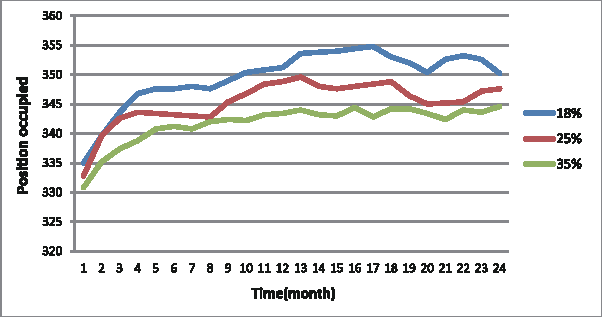
\includegraphics[width=10cm]{task4_p.pdf}\\
  \caption{Status of positions}\label{t4_p}
\end{figure}

To analyze the status of positions under different churn rate, we use our model to simulate dynamic processes with these churn rate constraints. We execute our program 100 times for each churn rate and average the predicted values. Figure \ref{t4_p} shows the averaged results our model predicted. Under all of these three conditions, the number of employees in the company keeps rising. The higher the churn rate, the lower the final full rate the company reaches after two years. But ICM can sustain its 80\% for positions even if the churn rate goes to 35\% according to our model's precition.

\begin{figure}[htb]
  \centering
  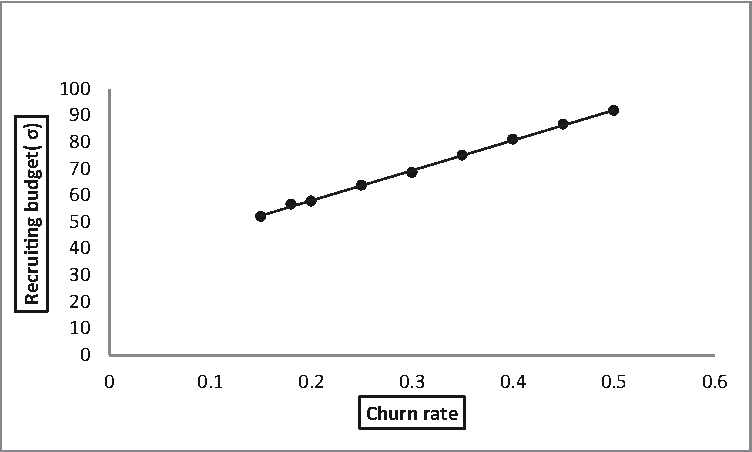
\includegraphics[width=10cm]{task4_r.pdf}\\
  \caption{Recruiting budget}\label{t4_r}
\end{figure}
\begin{figure}[htb]
  \centering
  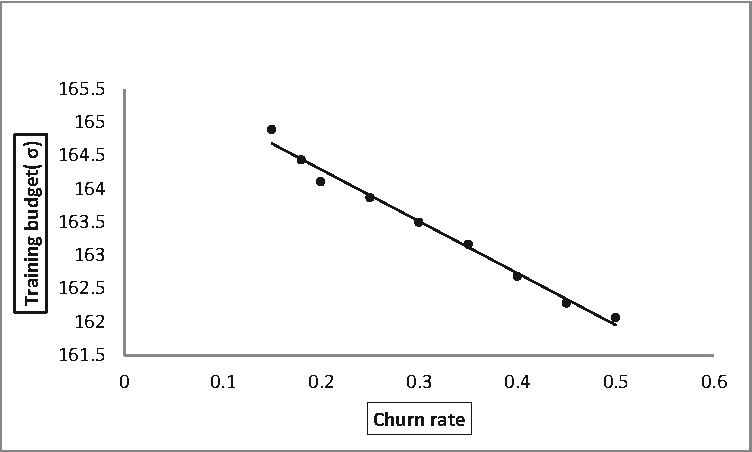
\includegraphics[width=7cm]{task4_t.pdf}
  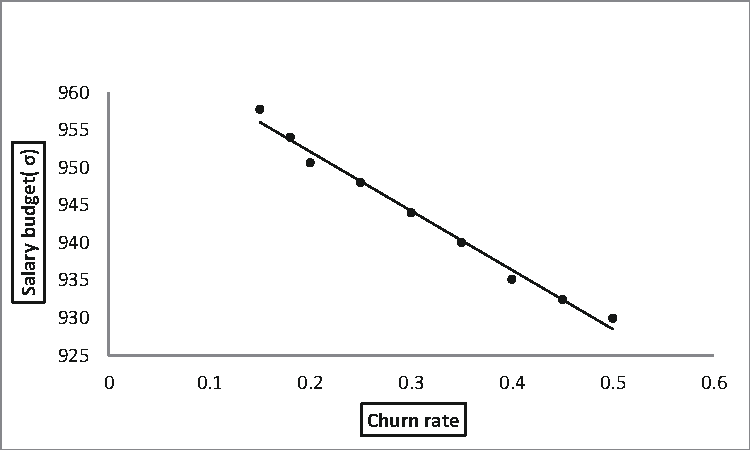
\includegraphics[width=7cm]{task4_s.pdf}\\
  \caption{Training budget and salary budget}\label{t4_t_s}
\end{figure}
The churn rate effect the budget of the company as well. The three parts of the bugdet behave differently when churn rate increases. The calculated budget is shown in Figure \ref{t4_r} and Figure \ref{t4_t_s}. Each data point in three charts is an averaged result of 10 predictions and a linear trendline is added to each chart. It is clear that recruiting budget showed in Figure \ref{t4_r} is likely to be proportional to the churn rate while salary budget and training budget showed in Figure \ref{t4_t_s} are likely to be inversely proportional to the churn rate.

To maintain enough employees, the company has to spend more on recruiting. So high turnover rate directly increase the recruiting budget. High turnover rate's effect on training budget and salary budget is more complex. On the one hand, when churn rate goes up, vacancies in the middle level keeps rising due to long recruiting time and low promote rate. On the other hand, the vacancies in lower level remains low because of the short recruiting time. So the full rate of the company decreases when churn rate rises. Since training budget and salary budget are closely related to full rate, both of them decrease when turnover rate goes up.
\subsection{Analysis for Task 5}
\label{sec:analysis-for-task-5}

\begin{figure}[htb]
  \centering
  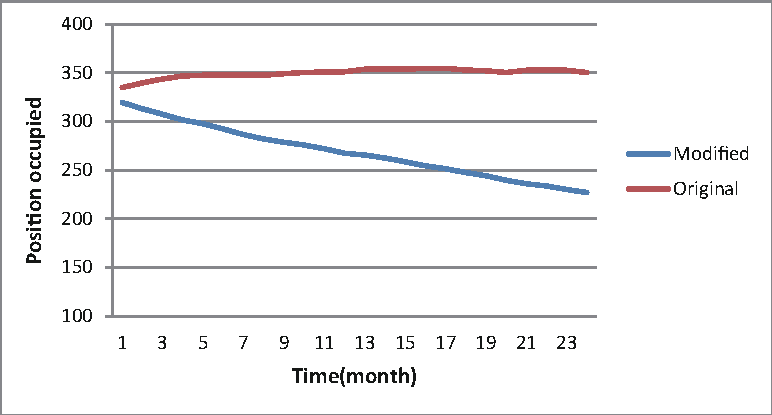
\includegraphics[width=10cm]{task5_p.pdf}\\
  \caption{Status of position}\label{t5_p}
\end{figure}
We apply following changes to our model to simulate the required process:\\
\begin{itemize}
\item Change the churn rate of junior managers and experienced supervisors to 30\%
\item Prohit external recruiting
\item Promoting only qualified employees
\end{itemize}
\begin{table}
	\begin{center}
		\begin{tabular}{l|cc}\toprule[2pt]
		\bfseries Level of Position & \bfseries Modified & \bfseries Original\\ \midrule
		Senior manager/Executive & 5.6 & 8.4\\
		Junior manager/Executive & 9.0 & 18.4\\
		Experienced supervisor & 7.4 & 23.0\\
		Inexperienced supervisor & 9.2 & 23.2\\
		Experienced employee & 72.6 & 107.4\\
		Inexperienced employee & 99.6 & 149.6\\
		Administrative clerk & 24.0 & 24.0\\ \bottomrule[2pt]
		\end{tabular}
		\caption{Status of position}\label{t5_p_t}
	\end{center}
\end{table}

The result of simulation is shown in Figure \ref{t5_p} and Table \ref{t5_p_t}. All the data shown is an average of ten predictions. While the number of positions occupied remains stable with origial conditions, it drops remarkably with modified conditions.

We list specific data of each level in Table \ref{t5_p_t}. In the modified case, the numbers of employees are lower than original case especially the those of middle levels. Since there is no external recruiting in modified case, it is obivious that the full rate will decrease due to employees' leave. Although some qualified employees can be promoted into higher level, the high churn rate of the middle level and difficulty of satisfying the promotion conditions make the numbers of middle level employees relatively low. The situation given in that task 5 will cause unrecoverable damage to ICM's HR health. With the full rate of middle level employees lower than 50\%, the HR structure is broken into fragments and the company won't be able to function normally.


\section{Advice for HR}
\label{sec:advice-for-hr}

a

\subsection{Incentive Mechanism}
\label{sec:incentive-machanism}

a

\subsection{Matching Employees to the Right Position}
\label{sec:matching-employees-to-the-right-position}

a

\section{Team Science}
\label{sec:team-science}

a

\section{Sensitivity Analysis}
\label{sec:sensitivity-analysis}

a

\section{Strengths and Weaknesses}
\label{sec:strengths-and-weaknesses}

\subsection*{Strengths}
\label{sec:strengths}

\begin{itemize}
\item Our model make fully use of the theory of multilayer networks so
  that it quantizes the relation accurately and reasonablly.
\item Our model exellently proves the interaction among these
  factors:leave probability, promotion probability and productivity.
\item The network we built include both microcosmic part and
  macrocosmic part, and they react to each other.
\item Our model proves the effection of time.
\end{itemize}

\subsection*{Weaknesses}
\label{sec:weaknesses}

\begin{itemize}
\item We assume that the water is still. In fact, streams flow and fluid dynamic is better taken into consideration. The actual situation is much complicated.
\item The model of the person should be more realistic. In fact, model of human body includes hands, legs or other parts, and the surface of human skin isn't even.
\item The condensation of water should be taken into consideration. Water that evaporate become water vapour, and some will condense into water on the bathtub.
\end{itemize}

\section{Conclusions}
\label{sec:conclusions}

a

% the reference
\begin{thebibliography}{99}

\bibitem{}

\end{thebibliography}

\label{LastPage}

\end{document}

%%% Local Variables:
%%% mode: latex
%%% TeX-master: t
%%% End:
